\graphicspath{{chapters/10/images/}}
\chapter{Protein profiles with HMMs}

\section{Introduction}
An alignment of two or more sequences can be used to infer the evolutionary relationships between sets of protein (or nucleic acid) sequences and eventually predict their 3D structure.
In order to obtain meaningful results, the accuracy of the alignment must be as high as possible.
Consider a family of protein sequences that all have a common three-dimensional structure, for example, the family of globins. A \textbf{profile} of globins can be thought of as a statistical model for the family of globins, in that for any sequence of amino acids, it defines a probability for that sequence, such that globin sequences tend to have much higher probabilities than non-globin sequences.
The aim of this paper is to build a class of structures related to profiles and propose them as statistical models of protein families, such that we are able to "learn" or "estimate" the stochastic model directly from raw unaligned sequences.
Once the model is obtained, it is possible to use it to discriminate sequences in the family from sequences not in the family, or to obtain a multiple alignment of all the sequences in the family to the model.
\\
\\
\noindent
The proposed method of multiple alignment is quite different from conventional methods, which are usually based on pairwise alignments using the standard dynamic programming scheme with gap penalties.
Such alignments often depend strongly on the particular values of the parameters required by the method, in particular the gap penalties. Furthermore, the same penalties are used for both fairly conserved regions and highly variable regions; substitutions, insertions, or deletions in a region of high conservation should ideally be penalized more than in a variable region.  The statistical model here proposed corresponds to multiple alignment with variable penalties, depending on the position and learned from the data itself.
\\
\\
\noindent
The type of statistical model is a hidden Markov model (HMM, or simply “model” for short). The HMM we build identifies a set of positions that describe the (more-or-less) conserved first-order structure in the sequences.
In biological terms, this corresponds to identifying the core elements of homologous molecules.
Each of these positions may be viewed as corresponding to a column in a multiple alignment of the sequences, or to a position in space, Often not all positions are modeled, but only the ones with the most significantly nonrandom statistics.
As in a profile, for each position in the model, the relative probabilities of the different amino acids in that position are given, as is the probability that the amino acid at that position is deleted. For any amino acid x,the negative logarithm of the probability of x at a given position in the model can be interpreted as a penalty for an alignment that puts z in this position, and the negative logarithm of the probability of deletion at that position can be similarly interpreted as a penalty for an alignment that puts a “ - ” (gap character) in that position. Furthermore, for each pair of adjacent positions, the model includes the probability for initiating an insertion of one or more amino acids between these positions, and the probability for extending it.
Other things are also included, such as the probability that an amino acid at a particular position is deleted, given that the amino acid at the previous position was deleted. This helps model the higher probability of consecutive deletions/insertions in certain regions. By taking negative logarithms as above, these methods provide a very flexible, position-dependent form of initiation and extension gap penalties.

\section{The protein HMM}
A hidden Markov Model describes a series of observations by a “hidden” stochastic process - a Markov process.
In this paper we are proposing an HMM similar to the ones used in speech to model protein families - or families of other molecular sequences like DNA and RNA. When modeling proteins, the observations are the amino acids in the primary sequence of a protein. A model for a set of proteins is one that assigns high probability to the sequences in that particular set.
\\
\\
\noindent
The HMM contains a sequence of $M$ states that we call match states. These correspond to positions in a protein or columns in a multiple alignment. Each of these states can generate a letter $x$ from the 20- letter amino acid alphabet according to a distribution $P(x|m_k), k= 1...M$.  For each match state $m_k$ there is a delete state $d_k$ that does not produce any amino acid, it is a “dummy” state, shown as circles. Finally, there are insertion states between all the match states, $M + 1$ in total, shown as diamonds. They generate amino acids in exactly the same way as the match states, but they use probability distributions $P ( x | i_k )$ .
From each state, there are three possible transitions to other states: transitions into match or delete states always move forward in the model, whereas transitions into insertion states do not. Multiple insertions between match states can occur because of the self loop on the insert state, meaning that a transition from an insert state to itself is possible. The transition probability from state $s_1$ to $s_2$ is called $\mathcal{T}(s_2|s_1)$.
The overall model is reported in figure \ref{fig:HMM}.

\begin{figure}[ht]
		\centering
		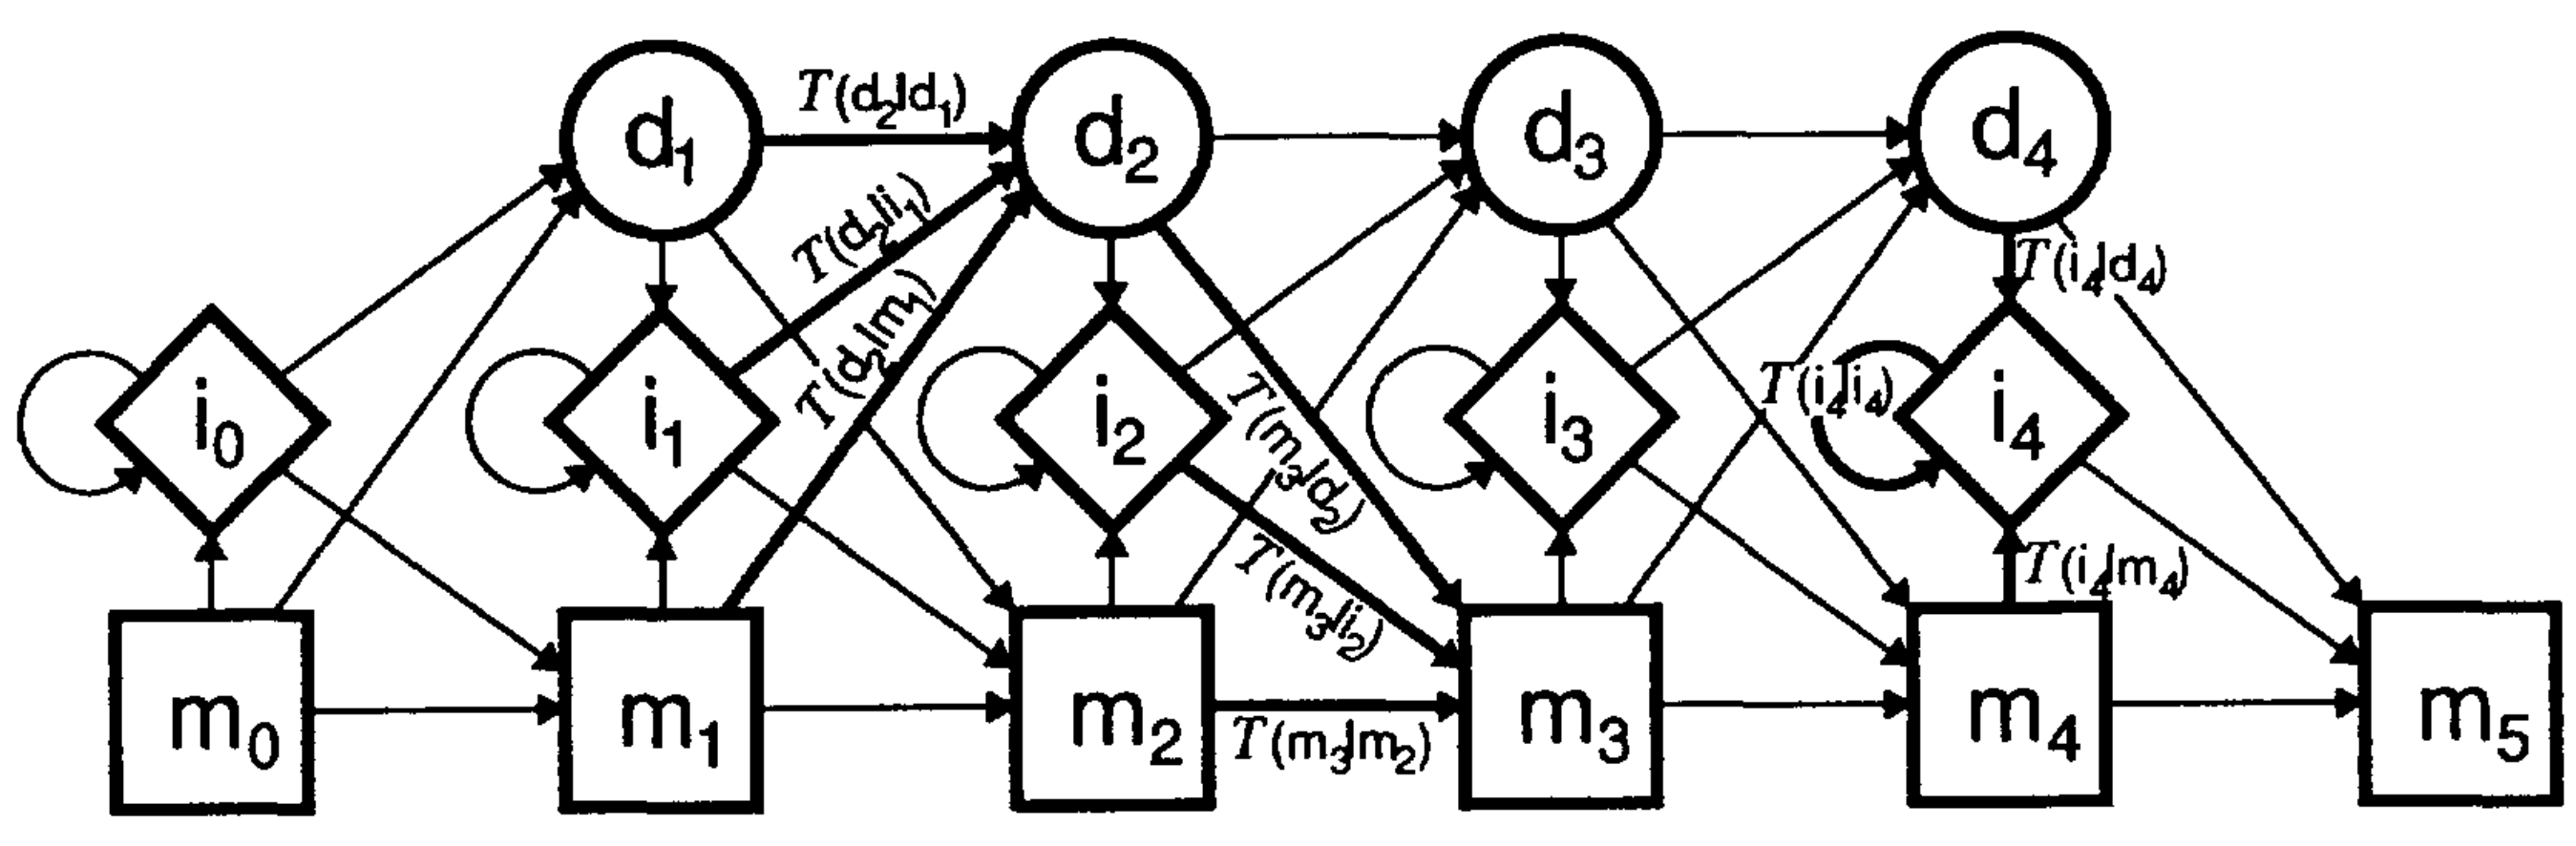
\includegraphics[width=0.5\textwidth]{HMM}
		\caption{\label{fig:HMM}}
	\end{figure}
\noindent
A sequence can be generated by a “random walk” through the model as follows: beginning at state $m_0$ (BEGIN) choose a transition  randomly according to the probabilities $\mathcal{T}(m_1|m_0),\mathcal{T}(d_1|m_0),\mathcal{T}(i_0|m_0)$. If $m_1$ is chosen, generate the first amino acid $x_1$ from the probability distribution $P(xlm_1)$, and choose a transition to the next state according to probabilities $\mathcal{T}(\cdot |m_1)$where $"\cdot"$ indicates any possible next state. Continue in this manner all the way to the END state, generating a sequence of amino acids $x_1, \dots, x_L$by following a path of states $y_0 \dots y_{N+1}$ through the model, where $y_0 = m_0$ (the BEGIN state) and $y{_N+1}=m_{M+1}$ (the END state). Because the delete states do not produce any amino acid, $N$ is larger than or equal to $L$.
\\
\\
\noindent
If $y_i$ is a match or insert state, we define $l(i)$ to be the index in the sequence $x_1, \dots, x_L$ of the amino acid produced in state $y_i$. The probability of the event that the path $y_{0} \dots y_{N+1}$ is taken and the sequence

\begin{equation}\label{eq:p_seq_path}
\operatorname{Prob}(x_1, \dots, x_L, y_0 \dots y_{N+1})= \mathcal{T}\left(m_{N+1} \mid y_{N}\right) \prod_{i=1}^{N} \mathcal{T}\left(y_{i} \mid y_{i-1}\right) \mathcal{P} (x_{l(i)}|y_i)
\end{equation}
where we set $\mathcal{P} (x_{l(i)}|y_i)=1$ if $y_i$ is a delete state. The probability of any sequence $x_1, \dots, x_L$ of amino acids is a sum over all possible paths that could produce that sequence]which we write as follows:
\begin{equation}\label{eq:p_seq}
\operatorname{Prob}(x_1, \dots, x_L)= \sum_{\text {paths}} \operatorname{Prob}(x_1, \dots, x_L, y_0 \dots y_{N+1})
\end{equation}
\noindent
In this way a probability distribution on the space of sequences is defined. The goal is to find a model that accurately describes a family of proteins by assigning large probabilities to sequences in that family.
\\
\\
\noindent
This structure for the HMM captures the structural intuition of a protein as a sequence of positions, each with its own distribution over the amino acids, along with the possibility for either skipping a position or inserting extra amino acids between consecutive positions, and allowing for the possibility that once a position is skipped, it may be more likely that positions following that one are also skipped. This choice appears to have worked well for modeling the globins,  but one can choose any structure for the states and transitions that is appropriate for the problem at hand.

\section{Estimating the HMM}
All the parameters in the model (i.e., probabilities) could in principle be chosen by hand from an existing alignment of protein sequences, or from information about the three-dimensional structure of proteins. The novel approach we take is to “learn” the parameters entirely automatically from a set of unaligned primary sequences, using an Expectation Maximization algorithm. The particular method we use to learn the model can be viewed as a computationally efficient approximation to Maximum A Posteriori (MAP) estimation of the parameters of the model.
\\
\\
\noindent
In MAP estimation,  the posterior probability is defined using Bayes rule,
\begin{equation} \label{eq:posterior}
\operatorname{Prob}(\text{model|sequences}) = \frac{\operatorname{Prob}(\text{sequences|model})\operatorname{Prob}(\text{model})}{\operatorname{Prob}(\text{sequences})}
\end{equation}
The prior on the models contains prior beliefs on what a model should be like, and can be used to “penalize” models that are known to be bad or uninteresting. To find the best model one can optimize the posterior probability \ref{eq:posterior} with respect to the parameters of the model.

\subsection{The distance from sequence to model}
First, we need a way to calculate the probability $\operatorname{Prob}(\text{sequences|model})$. Call the sequences $s^1 \dots s^n$.
Then, assuming independence
\begin{equation}\label{eq:p_seq_model}
\operatorname{Prob} (s^{1} \ldots s^{n} \mid \text { model }) = \prod_{\mu=1}^{n} \operatorname{Prob}(s^{\mu} \mid \text { model }) .
\end{equation}
\noindent
The expression for $\operatorname{Prob}(s^{\mu} |\text{model}) $ is given in can be calculated using the "forward algorithm". The previous equation can be approximated by the following for simplicity:
\begin{equation}\label{eq:p_s_model}
\operatorname{Prob}(s \mid \text { model }) \simeq \max _{\text {paths }} \operatorname{Prob}(s, \text{path } \mid \text { model})
\end{equation}
\noindent
Instead of maximizing the probability, it is most convenient to minimize the negative logarithm of the probability,  which is defined as the distance from the sequence to the model.
\begin{equation}\label{eq:p_s_model}
\text{ dist }(s, \text { model })=-\min _{\text {paths }} \log \operatorname{Prob}(s, \text { path } \mid \text { model }) =  -\min _{\text {paths }} \sum_{i=1}^{N+1}\left[\log \mathcal{T}\left(y_{i} \mid y_{i-1}\right)+\log \mathcal{P}\left(x_{l(i)} \mid y_{i}\right)\right)
\end{equation}

Where:
\begin{itemize}
\item path: $y_0 \dots y_{N+1}$
\item sequence $s$: $x_1 \dots x_L$
\item penalty: $\mathcal{T}\left(y_{i} \mid y_{i-1}\right)$
\end{itemize}
The penalties depends on the position in the model and the distance is very similar to the standard "edit distance" from one sequence to another. The most probable path can be found using the usual backtracking technique, as explained in the following section.

\subsection{Estimation algorithm}
The Baum-Welch or forward-backward algorithm is a version of the general EM (Expectation- Maximization) method often used in statistics, which can be applied faster but using the Viterbi approximation.
The Viterbi-EM adaptation of the model to the sequences is an iterative process.
It proceeds as follows:
\begin{enumerate}
\item choose the initial model
\item find the most probable path through the model for each of the sequences. The number of these paths that pass through state y is denoted $n(y)$, the number of times the transition from y to y' occurs $n(y'|y)$, and the number of times an amino acid $x$ was generated in state y is denoted $m(x|y)$. Obviously $n(m_k) = n(m_{k+1}|m_k)+n(d_{k+1} | m_k)+n(i_k|m_k)$ and similarly for delete and insert states
\item Reestimate the transition probabilities and amino acid probabilities in the match and insertion states from

\begin{equation}\label{eq:T}
\mathcal{T}\left(y^{\prime} \mid y\right) =\frac{n\left(y^{\prime} \mid y\right)+R\left(y^{\prime} \mid y\right)}{n(y)+\sum_{y^{\prime \prime}} R\left(y^{\prime \prime} \mid y\right)}
\end{equation}
\begin{equation}\label{eq:P}
\mathcal{P}(x \mid y) =\frac{m(x \mid y)+R(x \mid y)}{n(y)+\sum_{i=1}^{20} R\left(a_{i} \mid y\right)}
\end{equation}

Here $R(y'|y)$ and $R(x|y)$ represent a regularizer, which comes from the model prior \ref{eq:posterior} We assume that $R(y"|y) = 0$ if there is no transition from state $y$ to state $y"$. Often R is just set equal to one in order to avoid zero probabilities, but it can be used to bias the model in a certain direction.
\item repeat step 2 and 3 until the parameters change only insignificantly
\end{enumerate}
The main difference between this method, which uses the Viterbi approximation, and the standard Baum-Welch algorithm is that in the latter all paths (not just the most probable) are considered, but weighted according to their probability.

\subsection{Choosing the length of the model}
A simple heuristic selects a good model length, and even helps in the problem of local minima.
After learning, if more than a fraction $\gamma_{del}$ of the optimal paths of the sequences choose $d_k$, the delete state at position k,that position is removed from the model.
Similarly, if more than a fraction $\gamma_{ins}$ msake insertions at position k (in state $i_k$), a number of new positions are inserted into the model after position k. This number is equal to the average number of insertions the sequences make at that position. After these changes in the model, it is retrained, and this cycle is repeated until no more changes are needed. We call this “model surgery”. Currently we choose $\gamma_{del}$ and $\gamma_{ins}$ to be $1/2$.

\subsection{Over-fitting and regularization}
A model with too many free parameters cannot be estimated well from a relatively small data set of training sequences. If we try to estimate such a model, we run into the problem of overfitting.
One way to deal with this problem is to control the effective number of free parameters in the model by regularization, which can be viewed as a way of implementing MAP estimation.
In our application of regularization to HMMs, the regularizer is closely related to the model prior, and it can be used to bias the model in some specific direction. The regularizer ($R$)is added to the frequency counts in \ref{eq:T} and  \ref{eq:P} as if we actually saw more than $n(y’|y)$ or $n(x|y)$ events.
For instance, in our models we believe a prior $i$ that sequences should spend most of their time in the match states on the main line of the HMM, so we incorporate this belief into the model prior by setting $R(m_i|y)$to a large value compared to the regularizer $R(y|m_i)$,which is added to transitions diverging from the main line.
In so doing, these parameters become less adjustable, and as a result we are less prone to overfit the data.
We also tend to get better models because we are encouraging the learning algorithm to first explore the more a prior $i$ likely part of model space when trying to fit the data.
In the extreme case, the regularizers $R(\cdot | \cdot)$can be such large numbers that the parameters simply become “hardwired”. We have found that the method works best when very large regularizers $R(x|y)$, proportional to the relative overall frequencies of amino acids in globin sequences, are used when $y$ is an insert state. This has the effect of fixing the distributions in the insert states, rather than trying to estimate them from the training sequences.

\section{Conclusions}
The method utilizes the tremendous amount of information contained in many sequences from the same family.
For the simple case of globins, with this method it is possible to obtain multiple alignments that mirror structural alignments using only the unaligned primary sequences as input.
The method requires that many sequences be available from the family one wants to model; since the number of sequences in the protein databases is growing rapidly, this may be less of a problem in the future.
There are two possible answers to the problem of small sets of training sequences.
\\
\\
\noindent
The first is to add more prior knowledge into the training process by starting with a better initial model, and by using more involved kinds of regularization.
The "soft tying" regularization method combines the idea of tying states in which the number of free parameters is reduced by having groups of states all share the same distribution on the output alphabet (the 20 amino acids in this case), and the idea of soft weight, in which the regularizer (in this case for the distribution of amino acids) is also adaptively modified during learning.
Even more complex, position-specific kinds of regularization are possible.
Switching from the alphabet of the primary sequences to a different representation based more on the structural or chemical properties of the amino acids in the sequence may also help.
\\
\\
\noindent
The second answer is to give up trying to model the whole protein in cases where only few sequences are known, and instead try to model only pieces of the protein (motifs or domains) that have the same or similar structure in other proteins. In this case we can find more training sequences by adding in the corresponding pieces of these other proteins. In fact, the EM method can be used to locate the appropriate pieces by itself, given the entire sequences. Several models can also be linked together with free insertions in between, to model more than one subsequence in the molecules.
\\
\\
\noindent
Finally, when a relatively large number of sequences are available, it is sometimes possible to get better results by dividing these sequences into clusters of similar sequences, and training a different model for each cluster.
The partition into clusters can also be done automatically by the EM algorithm during training, in a procedure known as mixture modeling. To implement this, we simply start with more than one model and force the models to “compete” for the sequences, and adapt to fit only the ones they “won”.
